\begin{figure}[h]
	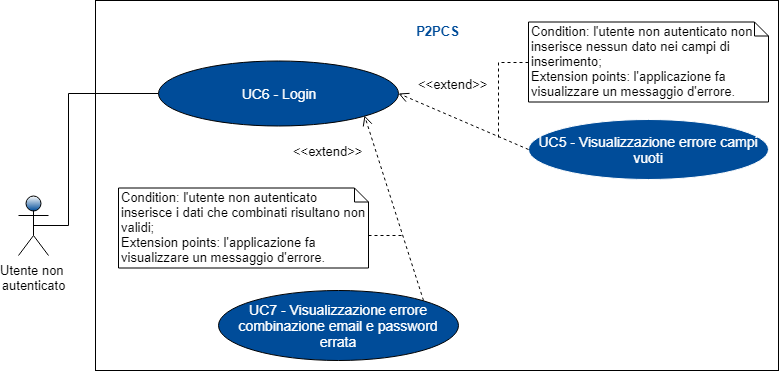
\includegraphics[width=16cm]{res/images/Schemagenerale2.png}
	\centering
	\caption{Diagramma del caso d'uso UC6 con relative estensioni (UC5, UC7)}
\end{figure}
\newpage
\subsubsection{UC6 - Login}
\begin{itemize}
	\item \textbf{Attori Primari}: utente non autenticato;
	\item \textbf{Descrizione}: per effettuare il procedimento di autenticazione, l'utente deve compilare i campi necessari e dopo averli confermati, se sono validi, verrà portato alla pagina di \textit{Gestione veicoli};
	\item \textbf{Scenario principale}: l'applicazione rende disponibili i campi da compilare per l'autenticazione. Dunque l'utente dovrà inserire tutti i dati necessari, quali:
	\begin{itemize}
		\item inserimento email [UC6.1];
		\item inserimento password [UC6.2].
	\end{itemize}
	successivamente conferma i dati inseriti;
	\item \textbf{Estensioni}:
	\begin{itemize}
		\item visualizzazione errore campi vuoti [UC5];
		\item visualizzazione errore combinazione email e password errata [UC7].
	\end{itemize}
	\item \textbf{Precondizione}: l'applicazione rende disponibile i campi da compilare;
	\item \textbf{Postcondizione}: dopo aver controllato che i campi sono stati compilati correttamente, l'utente viene autenticato nell'applicazione e rimandato alla pagina dei \textit{Gestione veicoli}.	
\end{itemize}
\begin{figure}[h]
	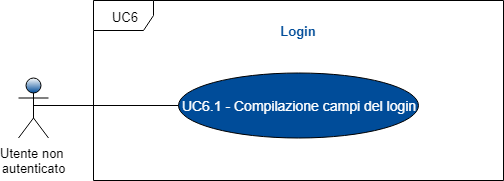
\includegraphics[width=11cm]{res/images/UC6Login.png}
	\centering
	\caption{UC6 - Login}
\end{figure}
\subsubsection{UC6.1 - Inserimento email}
\begin{itemize}
	\item \textbf{Attori Primari}: utente non autenticato;
	\item \textbf{Descrizione}: al fine di portare a termine il processo di autenticazione l'utente deve inserire l'indirizzo email associato all'account, campo ritenuto obbligatorio;
	\item \textbf{Scenario principale}: l'utente compila il campo relativo all'indirizzo email;	
	\item \textbf{Precondizione}: l'applicazione ha reso disponibile il campo per l'inserimento dell'indirizzo email;
	\item \textbf{Postcondizione}: l'utente ha compilato il campo con l'indirizzo email associato al proprio account.
\end{itemize}
\subsubsection{UC6.2 - Inserimento password}
\begin{itemize}
	\item \textbf{Attori Primari}: utente non autenticato;
	\item \textbf{Descrizione}: al fine di portare a termine il processo di autenticazione l'utente deve inserire la password associata al proprio account, campo ritenuto obbligatorio;
	\item \textbf{Scenario principale}: l'utente compila il campo relativo alla password;	
	\item \textbf{Precondizione}: l'applicazione ha reso disponibile il campo per l'inserimento della password;
	\item \textbf{Postcondizione}: l'utente ha compilato il campo con la password associata al proprio account.
\end{itemize}
\subsubsection{UC7 - Visualizzazione errore combinazione email e password errata}
\begin{itemize}
	\item \textbf{Attori Primari}: utente non autenticato;
	\item \textbf{Descrizione}: l'utente visualizza un messaggio d'errore in quanto i campi di inserimento email e password sono stati riempiti in modo errato;
	\item \textbf{Scenario principale}: l'utente non ancora autenticato tenta di accedere inserendo un indirizzo email e password che insieme risultano non validi;	
	\item \textbf{Precondizione}: l'utente non autenticato inserisce i dati che combinati risultano non validi;
	\item \textbf{Postcondizione}: l'applicazione fa visualizzare un messaggio d'errore.
\end{itemize}
\begin{figure}[h]
	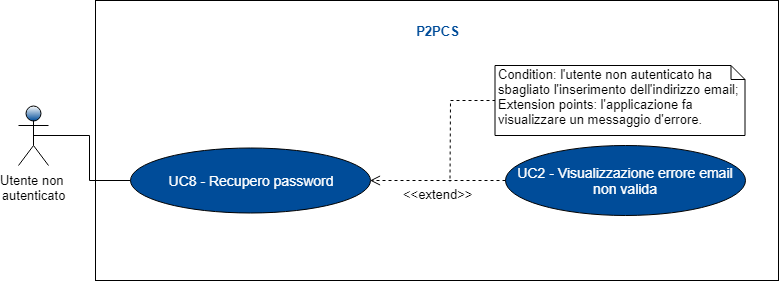
\includegraphics[width=15cm]{res/images/Schemagenerale3.png}
	\centering
	\caption{UC8 - Recupero password con relativa estensione (UC2)}
\end{figure}
\subsubsection{UC8 - Recupero password}
\begin{itemize}
	\item \textbf{Attori Primari}: utente non autenticato;
	\item \textbf{Descrizione}: l'utente non autenticato non si ricorda la propria password per accedere all'account e ne richiede il recupero che avviene inserendo un'indirizzo email dove verrà inviata una nuova password;
	\item \textbf{Scenario principale}: l'utente non ancora autenticato inserisce un'indirizzo email dove potrà ricevere la nuova password da utilizzare per accedere al proprio account;
	\item \textbf{Estensione}:
	\begin{itemize}
		\item visualizzazione errore email non valida [UC2].
	\end{itemize} 
	\item \textbf{Precondizione}: l'utente non autenticato non ricorda la password di accesso e indica un indirizzo email di recupero;
	\item \textbf{Postcondizione}: l'utente riceve la nuova password tramite posta all'indirizzo email inviato.
\end{itemize}
\subsubsection{UC9 - Logout}
\begin{figure}[h]
	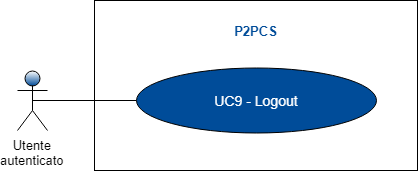
\includegraphics[width=9cm]{res/images/UC9Logout.png}
	\centering
	\caption{UC9 - Logout}
\end{figure}
\begin{itemize}
	\item \textbf{Attori Primari}:
	utente autenticato;
	\item \textbf{Descrizione}: l'utente dal fragment\glosp Area Personale richiede il logout dall'applicazione;
	\item \textbf{Scenario principale}: l'utente è autenticato nell'applicazione e richiede di effettuare il logout, premendo sull'apposito pulsante;
	\item \textbf{Precondizione}: l'utente ha effettuato il login all'applicazione e richiede di essere disconnesso dall'applicazione;
	\item \textbf{Postcondizione}: l'utente viene disautenticato e rimandato all'activity\glosp di login. 
\end{itemize}

